\documentclass{article}

\usepackage[a4paper, total={6in, 8in}]{geometry}
\usepackage{graphicx}
\graphicspath{ {./images/} }

\title{Incendio di un porto di mare}
\author{Eugenio Barbieri Viale, Leonardo Ippoliti}
\date{4D - a.s. 2024/2025}

\begin{document}
\setlength{\parindent}{0pt}
\maketitle

\begin{figure}[h]
    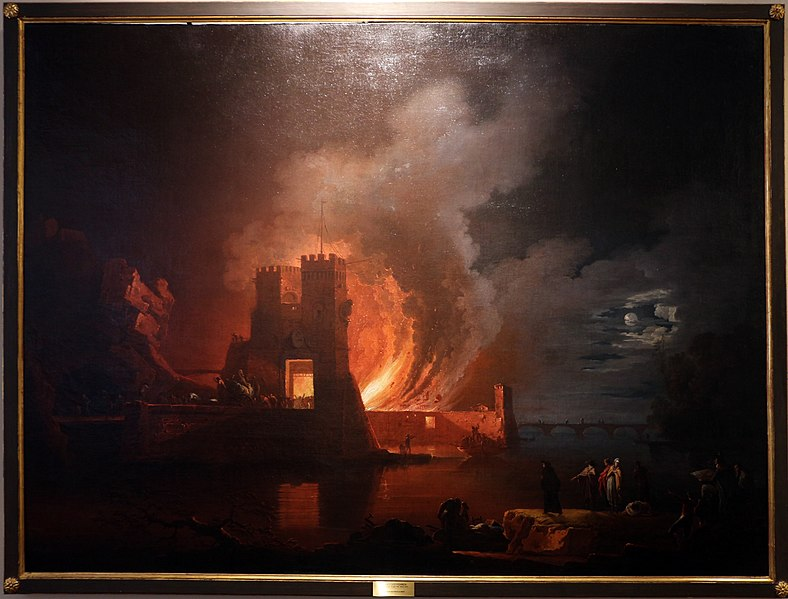
\includegraphics[scale=0.5]{dipinto1}
    \centering
\end{figure}

\begin{figure}[h]
    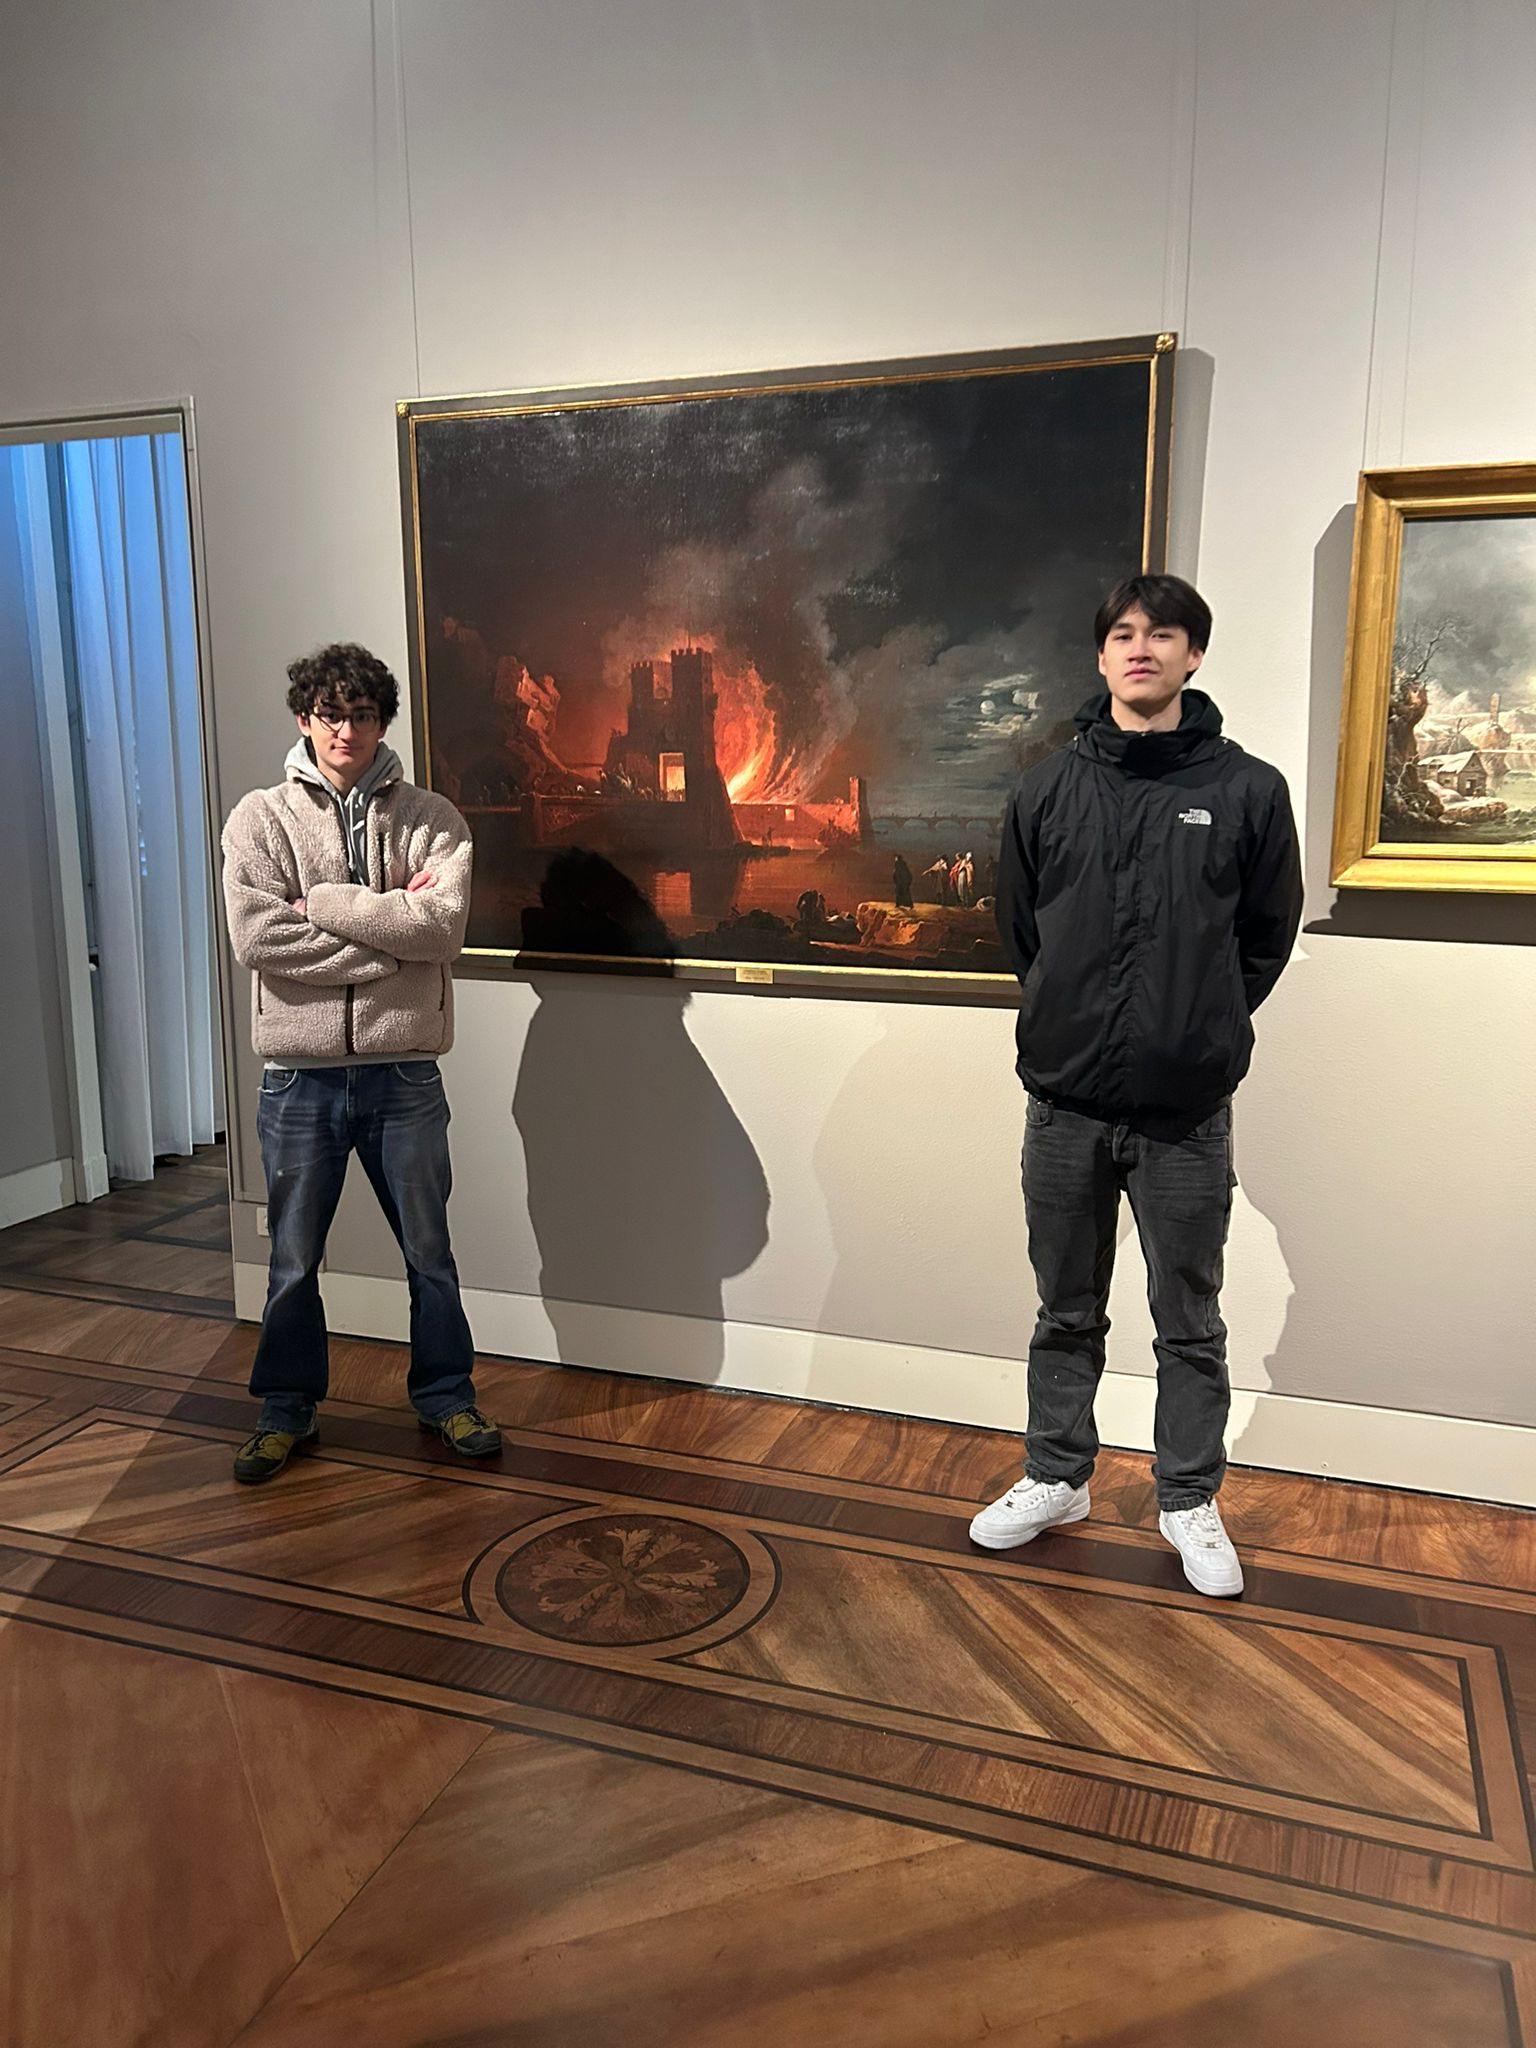
\includegraphics[scale=0.05]{selfie}
    \centering
\end{figure}

\section{L'artista - Francesco Fidanza}
Francesco Fidanza è un pittore romantico italiano e nasce a Roma nel 1747. Nel 1793 si trasferisce a Firenze, e nell'anno 1800 a Parigi. Qui probabilmente diventa allievo di \textit{Claude Joseph Vernet}, il quale influenza la sua pittura. Il pittore francese aveva infatti realizzato numerosi dipinti di porti per conto di Luigi XV.

\section{L'opera}
\subsection{Analisi iconografica}
\subsection{Analisi formale}
\subsection{Significato}

\end{document}

